\documentclass[10pt]{article}
\usepackage{icmlko}

\icmlmeta{IP 파운데이션 월드모델}{169}{한 칸이 얼마인지 안 정하고 다섯 노트를 썼다}{이진화가 공짜인지 보려다 섭동 크기가 열마다 뜻이 다르다는 것을 알았다. 고쳐서 다시 재니 노트 163의 $+$0.90이 $+$0.00이 된다}

\begin{document}

\twocolumn[
\icmlheader

\begin{abstract}
노트 168이 ``효과가 0 대 1$+$ 점프뿐이라면 이진으로 바꿔도 되나''를 남겼다.
바꿔 봤다. \textbf{판에서는 공짜다} --- 제작 주체 이력 축을 일곱 도메인에서
$\log_2(n{+}1)$ 눈금에서 이진 표지로 바꿔도 F18 배깅 $+$0.0034 $\pm$
0.0025($t{=}1.4$) · F6 능형 $+$0.0010 $\pm$ 0.0009($t{=}1.1$)로 \emph{안
갈린다}. 셈은 정보를 안 더한다. \textbf{그런데 손잡이 쪽에서 이상한 것이
나왔다} --- 이진화하니 그 축의 개입 효과가 F18 에서 0.0132에서
\textbf{0.0010}으로 떨어졌다. ``이진화가 축을 죽였다''로 읽을 뻔했다.
죽은 것은 축이 아니라 \textbf{재는 자}였다. 섭동을 0$\sim$4 척도의 한
칸이라는 뜻으로 \textbf{0.25 고정}으로 쓰고 있었는데, 이진 열(0/1)에 0.25를
밀면 트리는 분기(대개 0.5)를 못 넘어 예측이 한 비트도 안 변한다. 그래서
한 칸을 \textbf{그 열에서 관측된 값 사이의 중앙 간격}으로 고쳤다 --- 이진
열이면 1.0, $\log_2$ 계수 열이면 0.0425다. 고치니 이진 열의 효과가 0.0010
에서 0.0086으로 돌아오고 방향도 7/7이 된다. \textbf{그리고 다섯 노트가
흔들린다.} 고정 0.25로 잰 축별 크기와 관측 간격으로 잰 크기의 순위상관이
\textbf{$+$0.300}이다 --- 입장 마찰이 넷째에서 둘째로 올라온다. 그래서
노트 163의 핵심 --- ``축의 크기와 손잡이 정확도의 순위상관이
$+$0.900'' --- 을 다시 재니 \textbf{$+$0.000}이다. \textbf{크기 설명은
재는 자의 산물이었다.} 다만 정확도 자체는 거의 안 변한다(타깃 폭 100\% ·
굿즈 규모 98\% · 미디어 75\% · 장소 66\% · 마찰 65\%). 그러므로 무엇이
손잡이를 만드는가에 대한 설명은 하나만 남는다 --- \textbf{노트 164의
구성물 수}(순위상관 $-$0.632). 이 흐름에서 재는 자가 헤드라인을 뒤집은
것이 \textbf{네 번째}다.
\end{abstract}
]

\begin{figure*}[t]
\centering
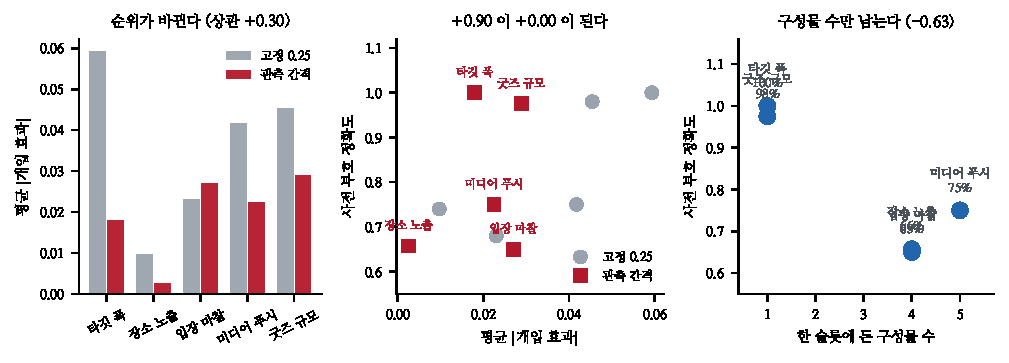
\includegraphics[width=\textwidth]{figs/step.pdf}
\caption{왼쪽 --- 축별 크기 순위가 바뀐다. 가운데 --- $+$0.90이 $+$0.00이
된다. 오른쪽 --- 구성물 수만 남는다.}
\end{figure*}

\section{이진화는 판에서 공짜다}

\begin{table}[t]
\centering\tsize
\caption{제작 주체 이력 축을 $\log_2(n{+}1)$ 에서 이진으로.}
\begin{tabular}{lrrl}
\toprule
& 판 $\rho$ 차 & 짝 sd & \\
\midrule
F18 배깅 & $+$.0034 & .0025 & $t{=}1.4$ 안 갈린다 \\
F6 능형 & $+$.0010 & .0009 & $t{=}1.1$ 안 갈린다 \\
\bottomrule
\end{tabular}
\end{table}

\claimx{\textbf{셈은 정보를 안 더한다.} 노트 167이 ``효과가 통째로 0 대
1$+$ 점프''라고 했고, 판에서도 그렇다 --- 몇 건인지는 안 쓰인다.}{그러니
코드가 $\log_2(n{+}1)$ 로 적어 둔 것은 뜻을 흐린다. 다만 되돌리는 값이
0이므로 급하지 않다.}

\section{그런데 재는 자가 걸렸다}

\claimx{\textbf{이진화하니 개입 효과가 0.0132에서 0.0010으로 떨어졌다.}
섭동을 ``0$\sim$4 척도의 한 칸''이라는 뜻으로 0.25 고정으로 쓰고 있었는데,
0/1 열에서 0.25를 밀면 트리 분기(대개 0.5)를 못 넘는다.}{``이진화가 축을
죽였다''로 읽을 뻔했다. 노트 156 · 160 · 166에서 세 번 겪은 모양이라 한
번 더 갈랐다.}

\begin{table}[t]
\centering\tsize
\caption{``한 칸''의 두 가지 뜻.}
\begin{tabular}{lrr}
\toprule
& 고정 & 관측 간격 \\
\midrule
$\log_2$ 계수 열 (모바일 · 펀딩) & .25 & \textbf{.0425} \\
이진 열 & .25 & \textbf{1.0} \\
\bottomrule
\end{tabular}
\end{table}

\claimx{\textbf{한 칸을 그 열의 관측 간격으로 고쳤다.} 이진 열의 효과가
0.0010에서 0.0086으로 돌아오고 방향이 7/7이 된다. F6 능형은 이진 열에
계수를 0으로 준다(0.0000) --- 그건 재는 자 문제가 아니라 그 모형이 안
쓰는 것이다.}{두 눈금이 서로 다른 질문에 답한다. 고정 0.25는 ``관측
범위의 4분의 1을 움직이면''이고 관측 간격은 ``한 단계 올리면''이다.
\textbf{다섯 노트가 앞엣것으로 쓰였다.}}

\section{그래서 노트 163이 흔들린다}

\begin{table}[t]
\centering\tsize
\caption{축별. 정확도는 거의 그대로, 크기는 바뀐다.}
\begin{tabular}{lrrrr}
\toprule
& \multicolumn{2}{c}{크기} & \multicolumn{2}{c}{정확도} \\
& 고정 & 간격 & 옛 & 새 \\
\midrule
타깃 폭 & .0593 & .0179 & 100\% & \textbf{100\%} \\
굿즈 규모 & .0454 & \textbf{.0288} & 98\% & \textbf{98\%} \\
미디어 푸시 & .0417 & .0224 & 75\% & 75\% \\
\textbf{입장 마찰} & .0230 & \textbf{.0270} & 68\% & 65\% \\
장소 노출 & .0097 & .0025 & 74\% & 66\% \\
\bottomrule
\end{tabular}
\end{table}

\claimx{\textbf{크기 순위가 바뀐다}(옛 대 새 순위상관 $+$0.300). 입장
마찰이 넷째에서 둘째로 올라오고 타깃 폭이 첫째에서 넷째로 내려간다.}{$\log_2$
계수 열은 관측 간격이 0.04로 촘촘하고 0$\sim$4 서수 열은 0.25다 --- 고정
스텝은 촘촘한 열에 여섯 배를 밀고 있었다.}

\claimx{\textbf{노트 163의 ``크기와 정확도의 순위상관 $+$0.900''이
$+$0.000이 된다.} 크기 설명은 재는 자의 산물이었다.}{정확도 자체는 거의
안 변한다 --- 타깃 폭 100\% · 굿즈 규모 98\%가 그대로고 장소 노출만
74\%에서 66\%로 내린다. \textbf{어느 축이 손잡이인가는 그대로고, 왜
그런가만 무너진다.}}

\claimx{\textbf{남는 설명은 노트 164의 구성물 수 하나다}(순위상관
$-$0.632). 구성물이 하나인 타깃 폭 · 굿즈 규모가 100\% · 98\%이고 넷$\sim$
다섯인 셋이 65$\sim$75\%다.}{노트 164가 ``구성물 수와 크기가 얽혀 있어
인과를 못 가른다''고 적었는데, 크기 쪽이 무너지면서 얽힘이 풀렸다.
\textbf{반증이 다른 가설을 확증한 셈이다.}}

\section{네 번째다}

\begin{table}[t]
\centering\tsize
\caption{이 흐름에서 재는 자가 헤드라인을 뒤집은 것.}
\begin{tabular}{lll}
\toprule
노트 & 무엇이 & 뒤집힌 것 \\
\midrule
156 & 순위 출력에 평균 차 & F10 ``역전 14\%'' \\
160 & 라벨로 정한 방향 & 입장 마찰 ``0/8'' \\
166 & 복제로 만든 공선성 & 제작사 이력 ``0/8'' \\
\textbf{169} & \textbf{열마다 다른 한 칸} & \textbf{크기 설명 $+$0.90} \\
\bottomrule
\end{tabular}
\end{table}

\claimx{\textbf{네 번 다 모형이 아니라 재는 자였다.} 그리고 네 번 다
``상식과 크게 어긋난다''가 신호였다.}{네 번을 다 잡았다는 뜻은 아니다 ---
잡은 것이 넷이다.}

\begin{table}[t]
\centering\tsize
\caption{남은 것.}
\begin{tabular}{ll}
\toprule
\textbf{두 눈금} & 고정과 간격 중 무엇이 손잡이의 뜻인가 \\
노트 163 & 크기 설명을 뺀 나머지는 유효 \\
이진화 & 판이 공짜니 코드도 이진으로 적을 것 \\
\bottomrule
\end{tabular}
\end{table}

첫 줄이 다음이다. 기획자가 돌리는 것은 ``관측 범위의 4분의 1''도 ``한
단계''도 아니고 \textbf{자기가 실제로 바꿀 수 있는 폭}이다. 팝업의 손 축
다섯은 0$\sim$4 서수라 ``한 등급''이 뜻이 있는데, 나머지 아홉 도메인의 유도
축은 그런 단위가 없다. \textbf{도메인마다 ``현실적인 한 걸음''을 정하는
것이 다음 일이다.}

\end{document}
